\chapter{Norm and Distance}

\section{Vector Norm}

\begin{definition}[Vector Norm]
    在向量空间中存在一个函数 $ \|\cdot\|: \mathbb{R}^{n} \rightarrow \mathbb{R} $, 且满足以下条件:

\begin{itemize}
    \item 齐次性: $ \|\alpha x\|=|\alpha|\|x\|, \quad \alpha \in \mathbb{R} $ 且 $ x \in \mathbb{R}^{n} $;
    \item 三角不等式: $ \|x+y\| \leq\|x\|+\|y\|, \quad x, y \in \mathbb{R}^{n} $;
    \item 非负性: $ \|x\| \geq {0}, {x} \in \mathbb{R}^{n} $ 且 $ \|{x}\|=0 \Leftrightarrow {x}=0 $;
\end{itemize}
则称$\|\cdot\|$为向量范数。 
\end{definition}







\subsection{$ \ell_{1} $-范数}

\begin{example}[$ \ell_{1} $-范数(曼哈顿范数,  Manhattan norm)]
    $$ \|x\|_{1}=\left|x_{1}\right|+\left|x_{2}\right|+\ldots+\left|x_{n}\right| \quad x, y \in \mathbb{R}^{n}, \alpha \in \mathbb{R} $$
\end{example}

\begin{proof}
    $$ \|\alpha x\|_{1}=\left|\alpha x_{1}\right|+\left|\alpha x_{2}\right|+\cdots+\left|\alpha x_{n}\right|=|\alpha|\|x\|_{1} \geq 0 $$

    $$ \|x+y\|_{1}=\left|x_{1}+y_{1}\right|+\cdots+\left|x_{n}+y_{n}\right| \leq\left|x_{1}\right|+\left|y_{1}\right|+\cdots+\left|x_{n}\right|+\left|y_{n}\right|=\|x\|_{1}+\|y\|_{1} $$
\end{proof}

\subsection{$ \ell_{2} $-范数}

\begin{example}[$ \ell_{2} $-范数(欧几里得范数, Euclidean norm)]
    $$ \|x\|_{2}=\sqrt{\left(x_{1}^{2}+x_{2}^{2}+\cdots+x_{n}^{2}\right)}=\sqrt{x^{T} x}=(\langle x, x\rangle)^{\frac{1}{2}} $$
\end{example}

\begin{proof}
    $$ \|\alpha x\|_{2}=(\langle\alpha x, \alpha x\rangle)^{\frac{1}{2}}=|\alpha|(\langle x, x\rangle)^{\frac{1}{2}}=|\alpha|\|x\|_{2} $$
    
    $$\begin{aligned} \|x+y\|_{2}^{2}&=\langle x+y, x+y\rangle 
    \\ &=\langle x, x\rangle+\langle x, y\rangle+\langle y, x\rangle+\langle y, y\rangle  \\
    &=\|x\|_{2}^{2}+2\langle x, y\rangle+\|y\|_{2}^{2} \leq\|x\|_{2}^{2}+2\|x\|_{2}\|y\|_{2}+\|y\|_{2}^{2}\\
    &=\left(\|x\|_{2}+\|y\|_{2}\right)^{2} \end{aligned}$$

    对于$$ \|x+y\|_{2} \leq\|x\|_{2}+\|y\|_{2} $$
    (for vectors $ a, b $ of equal size)

$$ \begin{array}{rlr}\|a+b\|^{2} & =(a+b)^{T}(a+b) & \\ & =a^{T} a+b^{T} a+a^{T} b+b^{T} b & \\ & =\|a\|^{2}+2 a^{T} b+\|b\|^{2} & \\ & \leq\|a\|^{2}+2\|a\|\|b\|+\|b\|^{2} \quad & \text { (by Cauchy-Schwarz) } \\ & =(\|a\|+\|b\|)^{2} & \end{array} $$



Note from line 3 that $ \|a+b\|^{2}=\|a\|^{2}+\|b\|^{2} $ if $ a^{T} b=0 $.
\end{proof}

\begin{corollary}
    Taking square-roots $ \|a+b\|^{2}=\|a\|^{2}+\|b\|^{2} $ gives the triangle inequality

    $$\| a + b \|_2 \le \|a \|_2 + \|b \|_2 $$

triangle inequality is an equality if and only if $ a^{T} b=\|a\|\|b\| $ .
\end{corollary}

\begin{corollary}[$ \ell_{2} $-Norm of block vector]
    If $ a, b $ are vectors,
$$
\left\|\left[\begin{array}{l}
a \\
b
\end{array}\right]\right\|_2 =\sqrt{\|a\|^{2}+\|b\|^{2}}
$$
\end{corollary}

\subsubsection{Cauchy–Schwarz inequality}

\begin{theorem}
    $$ \left|a^{T} b\right| \leq\|a\|\|b\| \quad \term{ for all } a, b \in \mathbf{R}^{n} $$
\end{theorem}

\begin{corollary}
    Moreover, equality $ \left|a^{T} b\right|=\|a\|\|b\| $ holds if:

\begin{itemize}
    \item $ a=0 $ or $ b=0 $; in this case $ a^{T} b=0=\|a\|\|b\| $
    \item $ a \neq 0 $ and $ b \neq 0 $, and $ b=\gamma a $ for some $ \gamma>0 $; in this case
    $$
    0<a^{T} b=\gamma\|a\|^{2}=\|a\|\|b\|
    $$

    \item $ a \neq 0 $ and $ b \neq 0 $, and $ b=-\gamma a $ for some $ \gamma>0 $; in this case
    $$
    0>a^{T} b=-\gamma\|a\|^{2}=-\|a\|\|b\|
    $$
\end{itemize}
\end{corollary}

\begin{proof}
    1. trivial if $ a=0 $ or $ b=0 $

2. assume $ \|a\|=\|b\|=1 $; we show that $ -1 \leq a^{T} b \leq 1 $
$$
\begin{array}{rlrl}
0 & \leq\|a-b\|^{2} & 0 & \leq\|a+b\|^{2} \\
& =(a-b)^{T}(a-b) & & =(a+b)^{T}(a+b) \\
& =\|a\|^{2}-2 a^{T} b+\|b\|^{2} & & =\|a\|^{2}+2 a^{T} b+\|b\|^{2} \\
& =2\left(1-a^{T} b\right) & & =2\left(1+a^{T} b\right)\\
 & \text{with equality only if }a=b &  & \text{with equality only if }a=-b
\end{array}
$$

3. for general nonzero $ a, b $, apply case 2 to the unit-norm vectors
$$
\frac{1}{\|a\|} a, \quad \frac{1}{\|b\|} b
$$
\end{proof}



\begin{corollary}[用$ \ell_{2} $范数表示的Cauchy-Schwarz(柯西—施瓦茨)不等式]
    $$ |\langle x, y\rangle|^{2} \leq\langle x, x\rangle\langle y, y\rangle=\|x\|_{2}^{2}\|y\|_{2}^{2} $$
\end{corollary}



\subsection{$ \ell_{\infty} $-范数}

\begin{definition}[$ \ell_{\infty} $-范数]
    $$ \|x\|_{\infty}=\max _{1 \leq i \leq n}\left|x_{i}\right|, x \in \mathbb{R}^{n} $$
\end{definition}

\begin{proof}
    $$ \begin{aligned} \max _{1 \leq i \leq n}\left|x_{i}\right| 
        &\leq \left(\left|x_{1}\right|^{p}+\cdots+\left|x_{i}\right|^{p}+\cdots+\left|x_{n}\right|^{p}\right)^{1 / p} \\
        &\leq \left(n \max _{1 \leq i \leq n}\left|x_{i}\right|^{p}\right)^{1 / p}\\
        &  =n^{1 / p} \max _{1 \leq i \leq n}\left|x_{i}\right| \\ &\rightarrow \max _{1 \leq i \leq n}\left|x_{i}\right| \quad(p \rightarrow \infty)\end{aligned}
    $$
\end{proof}

\subsection{$ \ell_{p} $-范数}

\begin{definition}[$ \ell_{\mathrm{p}} $-范数]
    $$ \|x\|_{p}=\left(x_{1}^{\mathrm{p}}+x_{2}^{p}+\cdots+x_{n}^{p}\right)^{\frac{1}{p}}, \quad x \in \mathbb{R}^{n}, p \ge 1 $$

    $ \ell_{1} $ 范数 $ \|x\|_{1}$,$ \ell_{2} $-范数 $ \|x\|_{2} $, $ \ell_{\infty} $-范数是 $ \ell_{p} $-范数的特例。 
\end{definition}

证明可以使用以下两条不等式

\begin{theorem}[Minkowski Inequality]
    $$ \left(\sum_{i=1}^{n}\left|x_{i}+y_{i}\right|^{p}\right)^{\frac{1}{p}} \leq\left(\sum_{i=1}^{n}\left|x_{i}\right|^{p}\right)^{\frac{1}{p}}+\left(\sum_{i=1}^{n}\left|y_{i}\right|^{p}\right)^{\frac{1}{p}}, p \geq 1, x, y \in \mathbb{R}^{n} $$
\end{theorem}

\begin{theorem}[Hölder Inequality]
    $$ \sum_{i=1}^{n}\left|x_{i} y_{i}\right| \leq\left(\sum_{i=1}^{n}\left|x_{i}\right|^{p}\right)^{1 / p}\left(\sum_{i=1}^{n}\left|y_{i}\right|^{q}\right)^{1 / q}, \frac{1}{p}+\frac{1}{q}=1,1<p, q<\infty $$
\end{theorem}

\section{Root Mean Square Value (RMS)}

\begin{definition}[向量 $ x $的均方值 (mean-square value)]
    向量 $ x \in \mathbb{R}^n $的均方值 (mean-square value)

    $$\operatorname{ms}(x) = \frac{x_{1}^{2}+x_{2}^{2}+\cdots+x_{n}^{2}}{n}=\frac{\|x\|_{2}^{2}}{n} $$
\end{definition}

\begin{definition}[n维向量 $ x $ 的均方根(root-mean-square value, RMS)]
    $$ \operatorname{rms}(x)=\sqrt{\frac{x_{1}^{2}+x_{2}^{2}+\cdots+x_{n}^{2}}{n}}=\frac{\|x\|_{2}}{\sqrt{n}} $$
\end{definition}

$ \operatorname{rms}(x) $ 给出了 $ \left|x_{i}\right| $ 的 “典型" (typical)值。 例如, $ \mathrm{rms}(\mathbf{1})=1 $ (与$n$无关). 均方根(RMS)值对于比较不同长度的向量大小是比较有用的。 

\begin{theorem}
    $$ |\operatorname{avg}(x)| \leq \operatorname{r m s}(x) $$
\end{theorem}

\section{Chebyshev's Inequality}

\begin{theorem}[Chebyshev's Inequality]
$$
\begin{aligned}
    P(|X-\mu| \ge \varepsilon) \le \frac{\sigma^2}{\varepsilon^2}
\end{aligned}
$$

$$
 P(|X-\mu| < \varepsilon) \ge 1 - \frac{\sigma^2}{\varepsilon^2}
$$
\end{theorem}

    

   
\begin{theorem}[Chebyshev's Inequality]
    假设$k$为向量 $ x $ 分量满足条件 $ \left|x_{i}\right| \geq a $ 的个数, 即 $ x_{i}^{2} \geq a^{2} $ 的个数。 

    则满足 $ \left|x_{i}\right| \geq a $ 的 $ x_{i} $ 数量$k$不会超过 $ \frac{\| x \|_{2}^{2}}{a^{2}} $.
\end{theorem}

\begin{proof}
    假设$k$为向量 $ x $ 分量满足条件 $ \left|x_{i}\right| \geq a $ 的个数, 即 $ x_{i}^{2} \geq a^{2} $ 的个数。
    
    因为有$k$个元素的平方$x_i^2$大于$a^{2}$,而$x_i^2$是非负的,所以有
    $$ \|x\|_{2}^{2}=x_{1}^{2}+x_{2}^{2}+\cdots+x_{n}^{2} \geq k a^{2} $$

    将 $ a^{2} $ 移项, 可得到 $ k \leq \frac{\|x\|_{2}^{2}}{a^{2}} $
\end{proof}

\begin{corollary}[Chebyshev's Inequality Using RMS]
    因为$ \operatorname{rms}(x)=\sqrt{\frac{x_{1}^{2}+x_{2}^{2}+\cdots+x_{n}^{2}}{n}}=\frac{\|x\|_{2}}{\sqrt{n}} $

    $ \left|x_{i}\right| \geq a $ 的项数占整体的比例不会超过 $ \left(\frac{\operatorname{rms}(x)}{a}\right)^{2} $, 即 $$ \frac{k}{n} \leq\left(\frac{\operatorname{rms}(x)}{a}\right)^{2} $$
\end{corollary}

\section{Distance}

\begin{definition}[Euclidean distance]
    $n$维向量$a$和$b$之间的欧氏距离
    $$ \operatorname{dist}(a, b)=\|a-b\|_{2} $$
\end{definition}

当n=1,2,3时,距离等同于\term{普通距离(ordinary distance)}.

\begin{theorem}
    $ \|a-b\| \geq 0 $ for all $ a, b $ and $ \|a-b\|=0 $ only if $ a=b $
\end{theorem}

\begin{definition}[RMS deviation]
    $ \operatorname{rms}(a-b) $ 是$a$和$b$之间的均方根偏差。
\end{definition}

\begin{corollary}
    RMS deviation between $ n $-vectors $ a $ and $ b $ is $ \operatorname{rms}(a-b)=\frac{\|a-b\|}{\sqrt{n}} $.
\end{corollary}

\begin{theorem}[Trianglar Inequality]
    $$ \|a-c\|_{2}=\|(a-b)+(b-c)\|_{2} \leq\|a-b\|_{2}+\|b-c\|_{2} \text{ for all } a, b, c $$
\end{theorem}

\begin{FigureCenter}{三角形边长}
    

    \tikzset{every picture/.style={line width=0.75pt}} %set default line width to 0.75pt        
    
    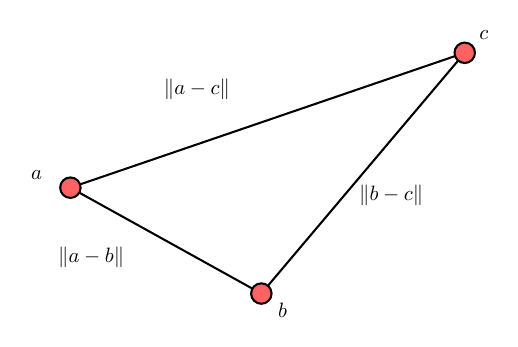
\begin{tikzpicture}[x=0.75pt,y=0.75pt,yscale=-1,xscale=1]
    %uncomment if require: \path (0,300); %set diagram left start at 0, and has height of 300
    
    %Straight Lines [id:da38129713930057973] 
    \draw    (238.07,177.93) -- (336.07,61.93) ;
    %Straight Lines [id:da5192962575960349] 
    \draw    (146.07,126.93) -- (336.07,61.93) ;
    %Straight Lines [id:da08930460970136278] 
    \draw    (238.07,177.93) -- (146.07,126.93) ;
    %Shape: Circle [id:dp482561418007299] 
    \draw  [fill={rgb, 255:red, 255; green, 98; blue, 98 }  ,fill opacity=1 ] (141.15,126.93) .. controls (141.15,124.21) and (143.35,122) .. (146.07,122) .. controls (148.79,122) and (151,124.21) .. (151,126.93) .. controls (151,129.65) and (148.79,131.85) .. (146.07,131.85) .. controls (143.35,131.85) and (141.15,129.65) .. (141.15,126.93) -- cycle ;
    %Shape: Circle [id:dp5528485613829361] 
    \draw  [fill={rgb, 255:red, 255; green, 98; blue, 98 }  ,fill opacity=1 ] (233.15,177.93) .. controls (233.15,175.21) and (235.35,173) .. (238.07,173) .. controls (240.79,173) and (243,175.21) .. (243,177.93) .. controls (243,180.65) and (240.79,182.85) .. (238.07,182.85) .. controls (235.35,182.85) and (233.15,180.65) .. (233.15,177.93) -- cycle ;
    %Shape: Circle [id:dp31125003972594856] 
    \draw  [fill={rgb, 255:red, 255; green, 98; blue, 98 }  ,fill opacity=1 ] (331.15,61.93) .. controls (331.15,59.21) and (333.35,57) .. (336.07,57) .. controls (338.79,57) and (341,59.21) .. (341,61.93) .. controls (341,64.65) and (338.79,66.85) .. (336.07,66.85) .. controls (333.35,66.85) and (331.15,64.65) .. (331.15,61.93) -- cycle ;
    
    % Text Node
    \draw (126,117.4) node [anchor=north west][inner sep=0.75pt]  [xscale=0.75,yscale=0.75]  {$a$};
    % Text Node
    \draw (245,181.33) node [anchor=north west][inner sep=0.75pt]  [xscale=0.75,yscale=0.75]  {$b$};
    % Text Node
    \draw (342,50.33) node [anchor=north west][inner sep=0.75pt]  [xscale=0.75,yscale=0.75]  {$c$};
    % Text Node
    \draw (190,73.4) node [anchor=north west][inner sep=0.75pt]  [xscale=0.75,yscale=0.75]  {$\| a-c\| $};
    % Text Node
    \draw (284.07,124.33) node [anchor=north west][inner sep=0.75pt]  [xscale=0.75,yscale=0.75]  {$\| b-c\| $};
    % Text Node
    \draw (139.07,154.33) node [anchor=north west][inner sep=0.75pt]  [xscale=0.75,yscale=0.75]  {$\| a-b\| $};
    
    
    \end{tikzpicture}
\end{FigureCenter}



\subsection{Feature Distance and Nearest Neighbor}

\begin{definition}[Feature Distance]
    如果 $ x $ 和y分别为两个实体的特征向量, 那么它们的特征距离(feature distance)为 $ \|x-y\|_{2} $
\end{definition}



\begin{definition}[Nearest Neighbor]
    给定向量$x$, 一个组向量$ z_{1}, \ldots, z_{m} $, 当$ \hat{q}_{j} $满足:

    $$ \left\|x-z_{j}\right\|_{2} \leq\left\|x-z_{i}\right\|_{2}, \quad i=1, \ldots, m $$

    则称 $ z_{j} $ 是 $ x $ 的\term{最近邻(nearest neighbor)}.
\end{definition}

\section{Standard Derivation}

\begin{definition}[算术平均值]
    对于$n$维向量$x$

    $$ \operatorname{avg}(x)=\frac{\mathbf{1}^{T} x}{n} $$
\end{definition}

\begin{definition}[De-meaned Vector]
    $$ \tilde{x}=x-\operatorname{avg}(x) \mathbf{1}\displaystyle =\left[\begin{array}{ c }
        x_{1} -\mathbf{avg} (x)\\
        x_{2} -\mathbf{avg} (x)\\
        \vdots \\
        x_{n} -\mathbf{avg} (x)
        \end{array}\right] =\left[\begin{array}{ c }
        x_{1} -\frac{\mathbf{1}^{T} x}{n} \ \\
        x_{2} -\frac{\mathbf{1}^{T} x}{n} \ \\
        \vdots \\
        x_{n} -\frac{\mathbf{1}^{T} x}{n} \ 
        \end{array}\right]$$

    因此 $ \operatorname{avg} (\tilde{x})=0 $
\end{definition}

\begin{definition}[$x$的标准差]
    $$\sigma= \operatorname{std}(x)=\operatorname{rms}(\tilde{x})=\frac{\left\|x-\left( \frac{1^{T} x}{n} \right) 1\right\|_{2}}{\sqrt{n}} $$
\end{definition}

$\operatorname{std}(x)$表示数据元素的变化程度。 对于常数$\alpha$, 当且仅当$ x=\alpha \mathbf{1} $时, $ \operatorname{std}(x)=0 $.

\begin{corollary}
    the de-meaned vector in standard units is
$$
\frac{1}{\operatorname{std}(a)}(a-\operatorname{avg}(a) \mathbf{1})
$$
\end{corollary}

\begin{theorem}
    $$ \operatorname{rms}(x)^{2}=\operatorname{avg}(x)^{2}+\operatorname{std}(x)^{2} $$
\end{theorem}

\begin{proof}
    $$\displaystyle \begin{aligned}
        \operatorname{std} (x)^{2} & =\frac{\| \mathbf{avg} (x)\mathbf{1} \| ^{2}}{n}\\
         & =\frac{1}{n}\left( x-\frac{\mathbf{1}^{T} x}{n}\mathbf{1}\right)^{T}\left( x-\frac{\mathbf{1}^{T} x}{n}\mathbf{1}\right)\\
         & =\frac{1}{n}\left( x^{T} x-\frac{\left(\mathbf{1}^{T} x\right)^{2}}{n} -\frac{\left(\mathbf{1}^{T} x\right)^{2}}{n} +\left(\frac{\mathbf{1}^{T} x}{n}\right)^{2} n\right)\\
         & =\frac{1}{n}\left( x^{T} x-\frac{\left(\mathbf{1}^{T} x\right)^{2}}{n}\right)\\
         & =\operatorname{rms} (x)^{2} -\operatorname{avg} (x)^{2}
        \end{aligned}$$
\end{proof}

\section{Angle}

\begin{definition}[两个非零向量 $ a $ 和$b$之间的角(angle)]
    $$ \angle(a, b)=\arccos \left(\frac{a^{T} b}{\|a\|_{2}\|b\|_{2}}\right) $$

    $ \angle(a, b) $ 的取值范围为 $ [0, \pi] $, 且满足$$ a^{T} b=\|a\|_{2}\|b\|_{2} \cos (\angle(a, b)) $$
\end{definition}

在二维和三维向量之中, 这里的角与普通角度(ordinary angle)是一致的。 

\begin{itemize}
    \item $\theta =\frac{\pi}{2}=90°$:a和b为正交, 写作$a \perp b (a ^T b  =0)$. 
    \item $\theta =0$:a和b为同向(aligned or parallel) $(a ^T  b=\| a \| \| b  \| )$. 
    \item $\theta =\pi =180°$: a和b为反向的(anti-aligned or opposed)$(a ^T   b  = - \| a \| \| b \| )$. 
    \item $\theta <\frac{\pi}{2}=90°$:a和b成锐角(acute angle)$(a ^T b >0)$. 
    \item $\theta >\frac{\pi}{2}=90°$:a和b成钝角(obtuse angle)$(a ^T b <0)$. 
\end{itemize}

\begin{theorem}
    Cauchy-Schwarz inequality guarantees that
$$
-1 \leq \frac{a^{T} b}{\|a\|\|b\|} \leq 1
$$
\end{theorem}

\begin{definition}[球面的距离]
    $$  \mathrm{R} \angle(a, b) $$
\end{definition}

\subsection{相关系数}

给定向量$a$和$b$, 其去均值向量为:

$$ \tilde{a}=a-\operatorname{avg}(a) 1,  \tilde{b}=b-\operatorname{avg}(b) 1 $$

\begin{definition}[$a$和$b$的相关系数]
    $$ \rho=\frac{\tilde{a}^{T} \tilde{b}}{\|\tilde{a}\|_{2}\|\tilde{b}\|_{2}} = \cos \angle (\tilde{a}, \tilde{b}) $$

    where  $ \tilde{a} \neq 0 $,  $ \tilde{b} \neq 0 $.
\end{definition}

It is only defined when $ a $ and $ b $ are not constant $ (\tilde{a} \neq 0 $ and $ \tilde{b} \neq 0) $, and is a number between $ -1 $ and $1$. $ \rho_{a b} $ is the cosine of the angle between the de-meaned vectors.

\begin{theorem}
    $ \rho_{a b} $ is the average product of the deviations from the mean in standard units
$$
\rho_{a b}=\frac{1}{n} \sum_{i=1}^{n} \frac{\left(a_{i}-\mathbf{a v g}(a)\right)}{\operatorname{std}(a)} \frac{\left(b_{i}-\mathbf{a v g}(b)\right)}{\operatorname{std}(b)}
$$
\end{theorem}


\begin{example}
    高度相关的向量:
\begin{itemize}
    \item 邻近地区的降雨时间序列。 
    \item 类型密切相关文档的单词计数向量。 
    \item 同行业中类似公司的日收益。 
\end{itemize}

比较不相关的向量:
\begin{itemize}
    \item 无关的向量。 
    \item 音频信号(比如, 在多轨录音中的不同轨). 
\end{itemize}

负相关的向量:
\begin{itemize}
    \item 深圳与墨尔本的每天气温变化
\end{itemize}
\end{example}

\section{Regression Line}

scatter plot shows two $ n $-vectors $ a, b $ as $ n $ points $ \left(a_{k}, b_{k}\right) $

straight line shows affine function $ f(x)=c_{1}+c_{2} x $ with
$$
f\left(a_{k}\right) \approx b_{k}, \quad k=1, \ldots, n
$$

\begin{problem}
    use coefficients $ c_{1}, c_{2} $ that minimize $$ J=\frac{1}{n} \sum_{k=1}^{n}\left(f\left(a_{k}\right)-b_{k}\right)^{2} $$

    $ J $ is a quadratic function of $ c_{1} $ and $ c_{2} $ :
$$
\begin{aligned}
J &=\frac{1}{n} \sum_{k=1}^{n}\left(c_{1}+c_{2} a_{k}-b_{k}\right)^{2} \\
&=  \dfrac{n c_{1}^{2}+2 n \operatorname{a v g}(a) c_{1} c_{2}+\|a\|^{2} c_{2}^{2}-2 n \operatorname{avg}(b) c_{1}-2 a^{T} b c_{2}+\|b\|^{2}}{ n}
\end{aligned}
$$
\end{problem}

to minimize $ J $, set derivatives with respect to $ c_{1}, c_{2} $ to zero:
$$
c_{1}+\operatorname{avg}(a) c_{2}=\operatorname{avg}(b), \quad n \operatorname{avg}(a) c_{1}+\|a\|^{2} c_{2}=a^{T} b
$$

\begin{theorem}
    solution is
$$
c_{2}=\frac{a^{T} b-n \operatorname{avg}(a) \operatorname{avg}(b)}{\|a\|^{2}-n \operatorname{avg}(a)^{2}}, \quad c_{1}=\operatorname{avg}(b)-\operatorname{avg}(a) c_{2}
$$
\end{theorem}

\begin{corollary}
    slope $ c_{2} $ can be written in terms of correlation coefficient of $ a $ and $ b $ :
$$
c_{2}=\frac{(a-\operatorname{avg}(a) \mathbf{1})^{T}(b-\operatorname{a v g}(b) \mathbf{1})}{\|a-\operatorname{a v g}(a) \mathbf{1}\|^{2}}=\rho_{a b} \frac{\operatorname{std}(b)}{\operatorname{std}(a)}
$$
\end{corollary}

Hence, 

\begin{corollary}
    expression for regression line can be written as
$$
f(x)=\operatorname{avg}(b)+\frac{\rho_{a b} \operatorname{std}(b)}{\operatorname{std}(a)}(x-\operatorname{avg}(a))
$$
\end{corollary}

\begin{corollary}
    correlation coefficient $ \rho_{a b} $ is the slope after converting to standard units:
$$
\frac{f(x)-\mathbf{a v g}(b)}{\operatorname{std}(b)}=\rho_{a b} \frac{x-\mathbf{a v g}(a)}{\operatorname{std}(a)}
$$
\end{corollary}



\section{Regression Model}


\begin{definition}[Regression Model]
    回归模型(regression model)为关于$x$的仿射函数
    $$ \hat{y}=x^{T} \beta+v $$

    $x$是\term{特征向量(feature vector)}, 它的元素$x_i$称为\term{回归元(regressors)}. $n$维向量 $ \beta $ 是\term{权重向量(weight vector)}. 标量 $ v $ 是\term{偏移量(offset)}. 标量 $ \hat{y} $ 是\term{预测值(prediction)}. 表示某个实际结果或因变量, 用$y$表示。 
\end{definition}

Recall the regression model

\begin{problem}
    $$
    \hat{y}=x^{T} \beta+v,
    $$
    where the $ n $-vector $ x $ is a feature vector for some object, $ \beta $ is an $ n $-vector of weights, $ v $ is a constant (the offset), and $ \hat{y} $ is the (scalar) value of the regression model prediction.
\end{problem}

Now suppose we have a set of $ N $ objects (also called \term{samples} or \term{examples}), with feature vectors $ x^{(1)}, \ldots, x^{(N)} $. The regression model predictions associated with the examples are given by
$$
\hat{y}^{(i)}=\left(x^{(i)}\right)^{T} \beta+v, \quad i=1, \ldots, N
$$

These numbers usually correspond to predictions of the value of the outputs or responses. If in addition to the example feature vectors $ x^{(i)} $ we are also given the actual value of the associated response variables, $ y^{(1)}, \ldots, y^{(N)} $, then our \term{prediction errors} or \term{residuals} are
$$
r^{(i)}=y^{(i)}-\hat{y}^{(i)}, \quad i=1, \ldots, N
$$

We can express this using \textbf{compact matrix-vector notation}. 

We form the $ n \times N $ feature matrix $ X $ with columns $ x^{(1)}, \ldots, x^{(N)} $. We let $ y^{\mathrm{d}} $ denote the $ N $-vector whose entries are the actual values of the response for the $ N $ examples. (The superscript `d' stands for `data'.) 

We let $ \hat{y}^{\mathrm{d}} $ denote the $ N $-vector of regression model predictions for the $ N $ examples, and we let $ r^{\mathrm{d}} $ denote the $ N $-vector of residuals or prediction errors. We can then express the regression model predictions for this data set in matrix-vector form as
$$
\hat{y}^{\mathrm{d}}=X^{T} \beta+v \mathbf{1}
$$

The vector of $ N $ prediction errors for the examples is given by
$$
r^{\mathrm{d}}=y^{\mathrm{d}}-\hat{y}^{\mathrm{d}}=y^{\mathrm{d}}-X^{T} \beta-v \mathbf{1} .
$$
We can include the offset $ v $ in the regression model by including an additional feature equal to one as the first entry of each feature vector:

\begin{problem}
    $$
\hat{y}^{\mathrm{d}}=\left[\begin{array}{c}
\mathbf{1}^{T} \\
X
\end{array}\right]^{T}\left[\begin{array}{l}
v \\
\beta
\end{array}\right]=\tilde{X}^{T} \tilde{\beta}
$$

where $ \tilde{X} $ is the new feature matrix, with a new first row of ones, and $ \tilde{\beta}=(v, \beta) $ is the vector of regression model parameters.
\end{problem}

 This is often written without the tildes, as $ \hat{y}^{\mathrm{d}}=X^{T} \beta $, by simply including the feature one as the first feature.

The equation above shows that the $ N $-vector of predictions for the $ N $ examples is a linear function of the model parameters $ (v, \beta) $. The $ N $-vector of prediction errors is an affine function of the model parameters.


\section{Norm for Complex Numbers}

\begin{definition}
    norm of vector $ a \in \mathbf{C}^{n} $ :
$$
\begin{aligned}
\|a\| &=\sqrt{\left|a_{1}\right|^{2}+\left|a_{2}\right|^{2}+\cdots+\left|a_{n}\right|^{2}} \\
&=\sqrt{a^{H} a}
\end{aligned}
$$
\end{definition}

\begin{theorem}
    [Positive definiteness]
$ \|a\| \geq 0 $ for all $ a, \quad\|a\|=0  $ only if $ a=0 $
\end{theorem}

\begin{theorem}
    [Homogeneous]
$ \|\beta a\|=|\beta|\|a\| $ for all vectors $ a $, complex scalars $ \beta $
\end{theorem}

\begin{theorem}
    [Triangle inequality]
$ \|a+b\| \leq\|a\|+\|b\| \quad $ for all vectors $ a, b $ of equal size
\end{theorem}

\begin{theorem}[Cauchy–Schwarz inequality for complex vectors]
    $ \left|a^{H} b\right| \leq\|a\|\|b\| \quad $ for all $ a, b \in \mathbf{C}^{n} $

    moreover, equality $ \left|a^{H} b\right|=\|a\|\|b\| $ holds if:

    \begin{itemize}
        \item $ a=0 $ or $ b=0 $
        \item $ a \neq 0 $ and $ b \neq 0 $, and $ b=\gamma a $ for some (complex) scalar $ \gamma $
    \end{itemize}
\end{theorem}

We say $ a $ and $ b $ are orthogonal if $ a^{H} b=0 $.

We will not need definition of angle, correlation coefficient, $ \ldots $ in $ \mathbf{C}^{n} $.
